Um sicher YouNow zu nutzen, können einfache Regeln beachtet werden. 

\paragraph{Wenig Profilinformationen}
Da es nicht erforderlich ist, sein Profil mit allen Informationen zu befüllen, sollte nur das nötigste angegeben werden. Wohnort und Kontaktdaten möglichst nicht ausfüllen. Außerdem sollte niemals der eigene Name als Nickname verwendet werden.


\paragraph{Informationen ausblenden}
Unter den Profileinstellungen kann man die Option \textit{hide my city} anklicken. Dadurch wird der Wohnort verborgen. (siehe \ref{privats_einstellung})

\begin{figure}[!ht]
\centering
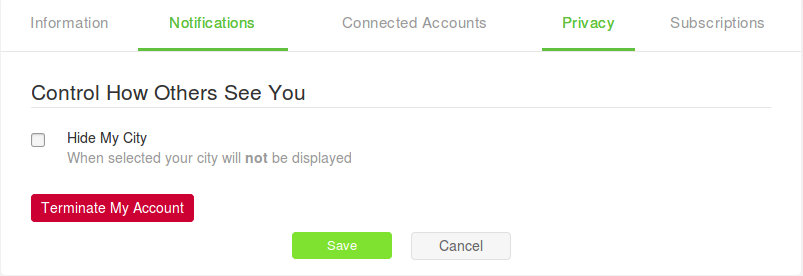
\includegraphics[width=0.6\textwidth]{./resources/younow_hide_my_city}
\caption{Einstellungen für die Privatsphäre}
\label{privats_einstellung}
\end{figure} 

\paragraph{Nutzer melden/blockieren}
Sind Personen aufdringlich oder beleidigend, kann man diese blockieren, sodass sie dann keine Möglichkeit mehr haben, Kontakt aufzunehmen. Allerdings gilt das nur für angemeldete Nutzer. Der Live-Stream ist weiterhin für jedermann zugänglich.
Möchte man einen anderen Nutzer melden, weil er gegen eines der YouNow Regeln verstoßen hat, kann man dies über die Melde-Funktion machen. Eine weitere Option besteht darin, direkt Kontakt mit einem Moderator aufzunehmen. Hierbei gibt es ein Kontaktformular. Hier müssen Angaben wie der Grund, eine Beschreibung und ggf. ein Screenshots angeben.

\paragraph{Antworten vorbereiten}
Während eines Live-Streams werden die Streamenden oft nach dem Alter, Wohnort bzw. Adresse oder anderen persönlichen Fragen gefragt. Hier empfiehlt es sich, vorab darüber nachzudenken, wie man darauf antworten könnte. So kann bei der Frage nach dem Wohnort bzw. Adresse eine sehr ungenaue Antwort wie: \glqq Ich komme aus Bayern\grqq geantwortet werden. Und bei weiteren Nachfragen könnte man bestimmt antworten: \glqq Genauer möchte ich nicht darauf eingehen\grqq .
Weiter kann man sich die eigene häusliche Umgebung für den Live-Stream gut ansehen und persönliche Dinge in dem Zimmer entfernen bevor man den Stream startet. 
